% ============================================================================
% 第 4 章 系统总体设计
% 预估页数：4 页
% 写作总要点：
%   - 重点是 "架构思想"，不是代码
%   - 每个核心架构图都要有，再用一段文字解读
% ============================================================================
\chapter{系统总体设计}

% ----------------------------------------------------------------------------
\section{系统架构设计}

\subsection{整体架构}
% 写作要点：
%   - 五层架构：用户层 / 接入层（Nginx）/ 应用层（前后端）/ 数据层 / AI 服务层
%   - 用一张图表达分层（figures/architecture\_overall.png）
%   - 解读每一层的作用与边界

本系统采用“用户层—接入层—应用层—AI 服务层—数据层”五层架构进行设计，各层之间以标准化协议交互，职责边界清晰，便于独立迭代与水平扩展。系统整体架构如图~\ref{fig:architecture_overall} 所示。
用户层作为架构的最外层，包含学生、教师与管理员三类使用者，以主流浏览器为接入终端；接入层由 Nginx 反向代理服务构成，负责静态资源下发、路由分发、HTTPS 终结与跨域控制。应用层包括 Vue 3 前端应用与 Spring Boot 后端服务两个子部分：前端以静态资源形式部署于 Nginx，后端以 Spring Boot 应用运行在独立容器中，对外提供 RESTful API 与 SSE 接口。AI 服务层是本系统区别于传统教学系统的核心抽象，包含 Agent 路由、RAG 检索、会话记忆、工具调用与评分兜底五个模块，是介于应用层与外部大语言模型之间的领域中层。数据层采用 MySQL 存储业务数据、Redis 存储会话与缓存、MinIO 存储医学影像与文档附件，外部 AI 服务以 SaaS 方式调用阿里云百炼提供的通义千问模型。这种分层设计的优势在于：各层只依赖于下一层的对外接口，可以独立选择实现、独立部署；AI 服务层的抽象为后续替换模型、添加多模型路由与增加本地部署模型预留了扩展点。

\begin{figure}[H]
    \centering
    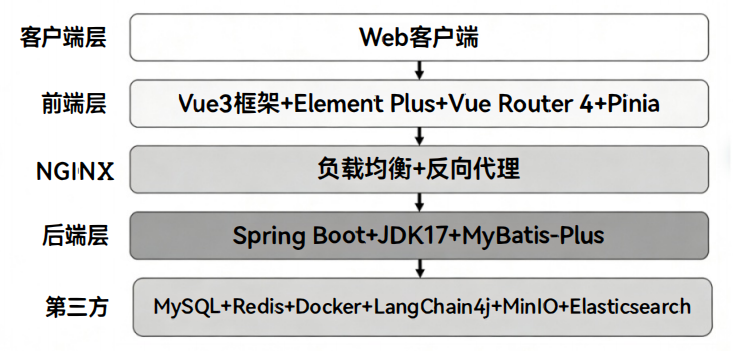
\includegraphics[width=0.85\textwidth]{figures/整体架构图.png}
    \caption{系统整体架构图}
    \label{fig:architecture_overall}
\end{figure}

\subsection{前后端分离架构}
% 写作要点：
%   - 前端：Vue3 + Vite，构建为静态资源，通过 Nginx 托管
%   - 后端：Spring Boot，提供 RESTful API + WebSocket
%   - 通信：HTTPS + JWT
%   - 优势：开发解耦、独立部署、可扩展

上述架构中的应用层采用严格的前后端分离设计。前端以 Vue 3 + TypeScript + Element Plus 为技术选型，使用 Vite 作为构建与开发服务器，所有页面在构建后以 \texttt{dist/} 静态资源的形式交由 Nginx 托管。后端以 Spring Boot 3.3.6 为核心运行环境，对外提供两类接口：一是遵循 REST 风格的业务接口，以 \texttt{/api/<资源>/<动作>} 的路由约定与统一响应体返回业务数据；二是面向 AI 多轮对话场景的 SSE 流式接口，以 \texttt{text/event-stream} 进行字粒级推送。

前后端之间的路由交给 Nginx 处理：前端资源以 \texttt{/} 作为路径前缀，后端接口以 \texttt{/api/} 作为前缀转发到 Spring Boot 实例的 8081 端口，SSE 接口则将 \texttt{proxy\_buffering} 关闭以保证实时推送。身份认证采用 JWT 令牌机制，前端在 \texttt{Authorization} 请求头中携带 \texttt{Bearer <token>}，后端通过过滤器进行验证与上下文注入。这种架构使前后端可以独立迭代与部署，同时为后续推出移动端、桌面端与开放 API 预留了扩展空间。

\subsection{多 Agent 协同架构}
% 写作要点：
%   - 这一节是为第 5 章铺垫
%   - 一段简介："本系统在 LLM 之上构建了 Agent 编排层"
%   - 给出 Agent 协同总图：
%       学生消息 → AgentRouter → PatientAgent / DiagnosisAgent / FeedbackAgent
%               ↓
%             RAG 知识 + Memory 上下文 + Tool 工具调用
%               ↓
%             LLM (Qwen) → 流式响应

为避免在同一个提示词中同时负责“扮演病人”与“评估学生”带来的角色混淆问题，本系统在大语言模型之上构建了一个轻量级的 Agent 编排层。如图~\ref{fig:architecture_agent} 所示，学生发送的消息先进入 \texttt{AgentRouter}，路由器根据当前训练阶段与消息类型在三个领域 Agent（PatientAgent、DiagnosisAgent、FeedbackAgent）中选择一个最合适的实体；被选中的 Agent 提供专属的 \texttt{AgentProfile}（包含系统提示词与温度参数），并与三个横向能力模块联动：KnowledgeRAGService 从知识库中检索与话题相关的医学知识点；ConversationMemoryService 从 Redis 中恢复多轮上下文；AiToolService 在必要时以 Function Calling 形式调用临床工具。

\begin{figure}[H]
    \centering
    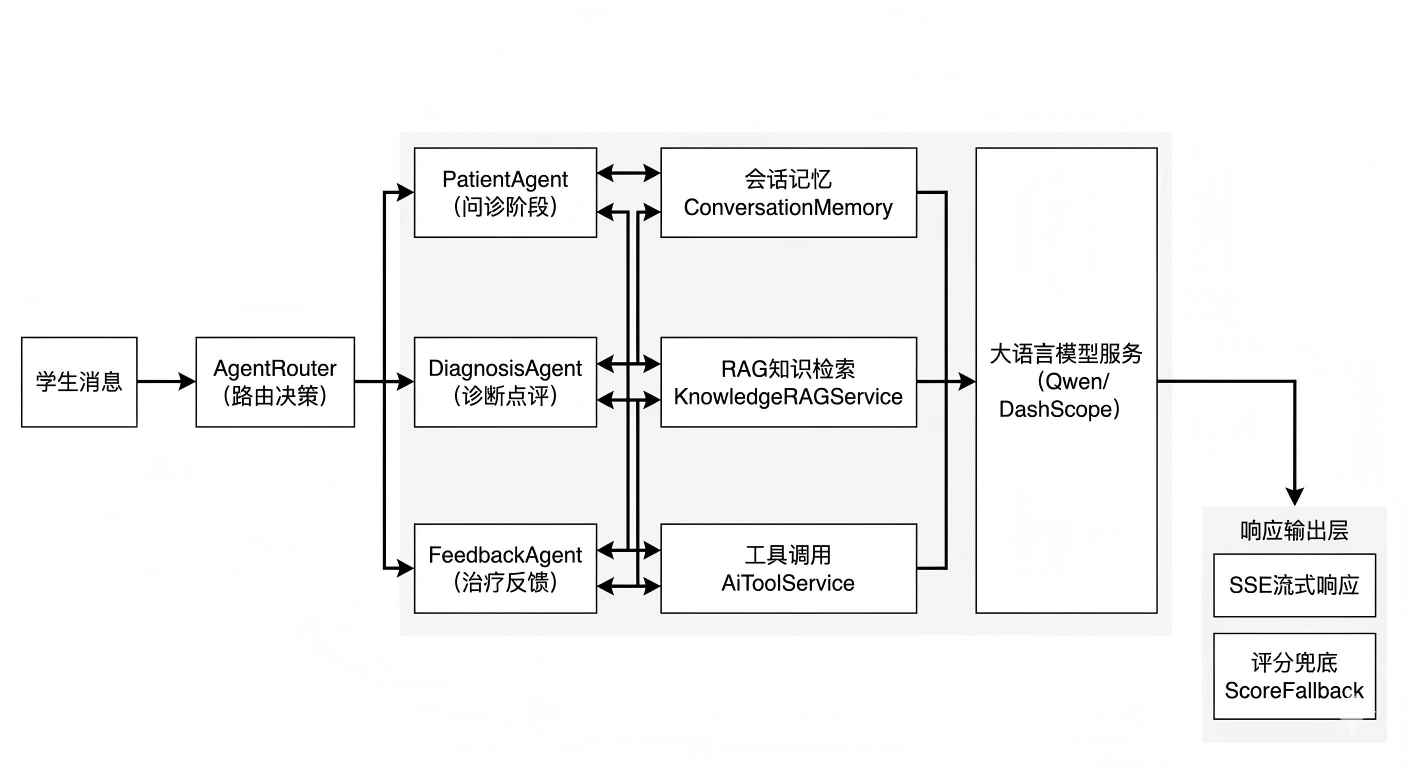
\includegraphics[width=0.85\textwidth]{figures/多Agent协同架构示意图.png}
    \caption{多 Agent 协同架构示意图}
    \label{fig:architecture_agent}
\end{figure}

在获得上下文后，Agent 层将完整提示词提交给外部的大语言模型服务（DashScope / Qwen），后者以 SSE 流式响应返回生成结果。返回后的话术同时被三者消费：一是被转发给前端以实现逐字输出；二是被写入训练对话表（\texttt{training\_dialog}）永久存储；三是被追加到 Memory 中作为下一轮对话的上下文。在训练结束提交阶段，AgentRouter 切换到 DiagnosisAgent 与 FeedbackAgent，并调用 \texttt{AiService.evaluateTraining()} 以结构化 JSON 形式输出多维评分；若 JSON 解析失败则触发规则兜底（ScoreFallback），生成保底评分以保证服务可用性。该架构作为本系统的核心创新点，在第 5 章中将进行详细实现说明。

% ----------------------------------------------------------------------------
\section{功能模块划分}
系统功能模块按照“使用角色 + 公共能力 + AI 核心能力”的方式划分。学生端围绕训练闭环展开，教师端围绕病例资源与教学评价展开，管理员端围绕系统运行与权限治理展开，公共模块为三类用户提供统一认证、消息、文件与可视化能力，AI 核心模块则作为横向能力被学生训练、教师批改与学习分析复用。
学生端的核心业务是完成一次可复盘的 AI 问诊训练，因此其模块包括病例浏览、训练启动、多轮问诊、诊断与治疗提交、训练报告、学习分析和个人中心。教师端负责教学资源供给与结果反馈，包括病例管理、班级管理、成绩管理、批改工作台、教学分析和通知管理。管理员端负责系统治理，包括用户管理、角色权限、系统监控、操作日志、存储管理和基础数据维护。公共模块包括 JWT 登录认证、验证码、文件上传、消息通知、统一异常与接口响应。AI 核心模块包括 Agent 路由、RAG 知识检索、Redis 会话记忆、临床工具调用和结构化评分。该划分方式保证了业务边界清晰，同时也便于后续按照模块进行独立开发、测试和部署。


% ----------------------------------------------------------------------------
\section{数据库设计}

\subsection{ER 图}
数据库设计以“用户—病例—训练—评分”为主线，并向教学班级、知识点、权限与日志扩展。核心实体包括用户表 \texttt{sys\_user}、角色表 \texttt{sys\_role}、病例表 \texttt{case\_info}、病例内容表 \texttt{case\_content}、训练记录表 \texttt{training\_record}、训练对话表 \texttt{training\_dialog}、训练评分表 \texttt{training\_score}、知识点表 \texttt{knowledge\_point}、班级表 \texttt{class\_info} 及班级学生关联表 \texttt{class\_student}。其中，用户与角色是一对多关系；教师用户创建病例，学生用户基于病例产生训练记录；每条训练记录可对应多轮对话与一条结构化评分记录；病例与知识点通过 \texttt{case\_knowledge} 形成多对多关系，用于支撑 RAG 检索与学习薄弱点分析；班级与学生通过关联表建立多对多关系，用于教师端班级统计和成绩批改。系统核心数据库 ER 图如图~\ref{fig:er_diagram} 所示。

\begin{figure}[H]
    \centering
    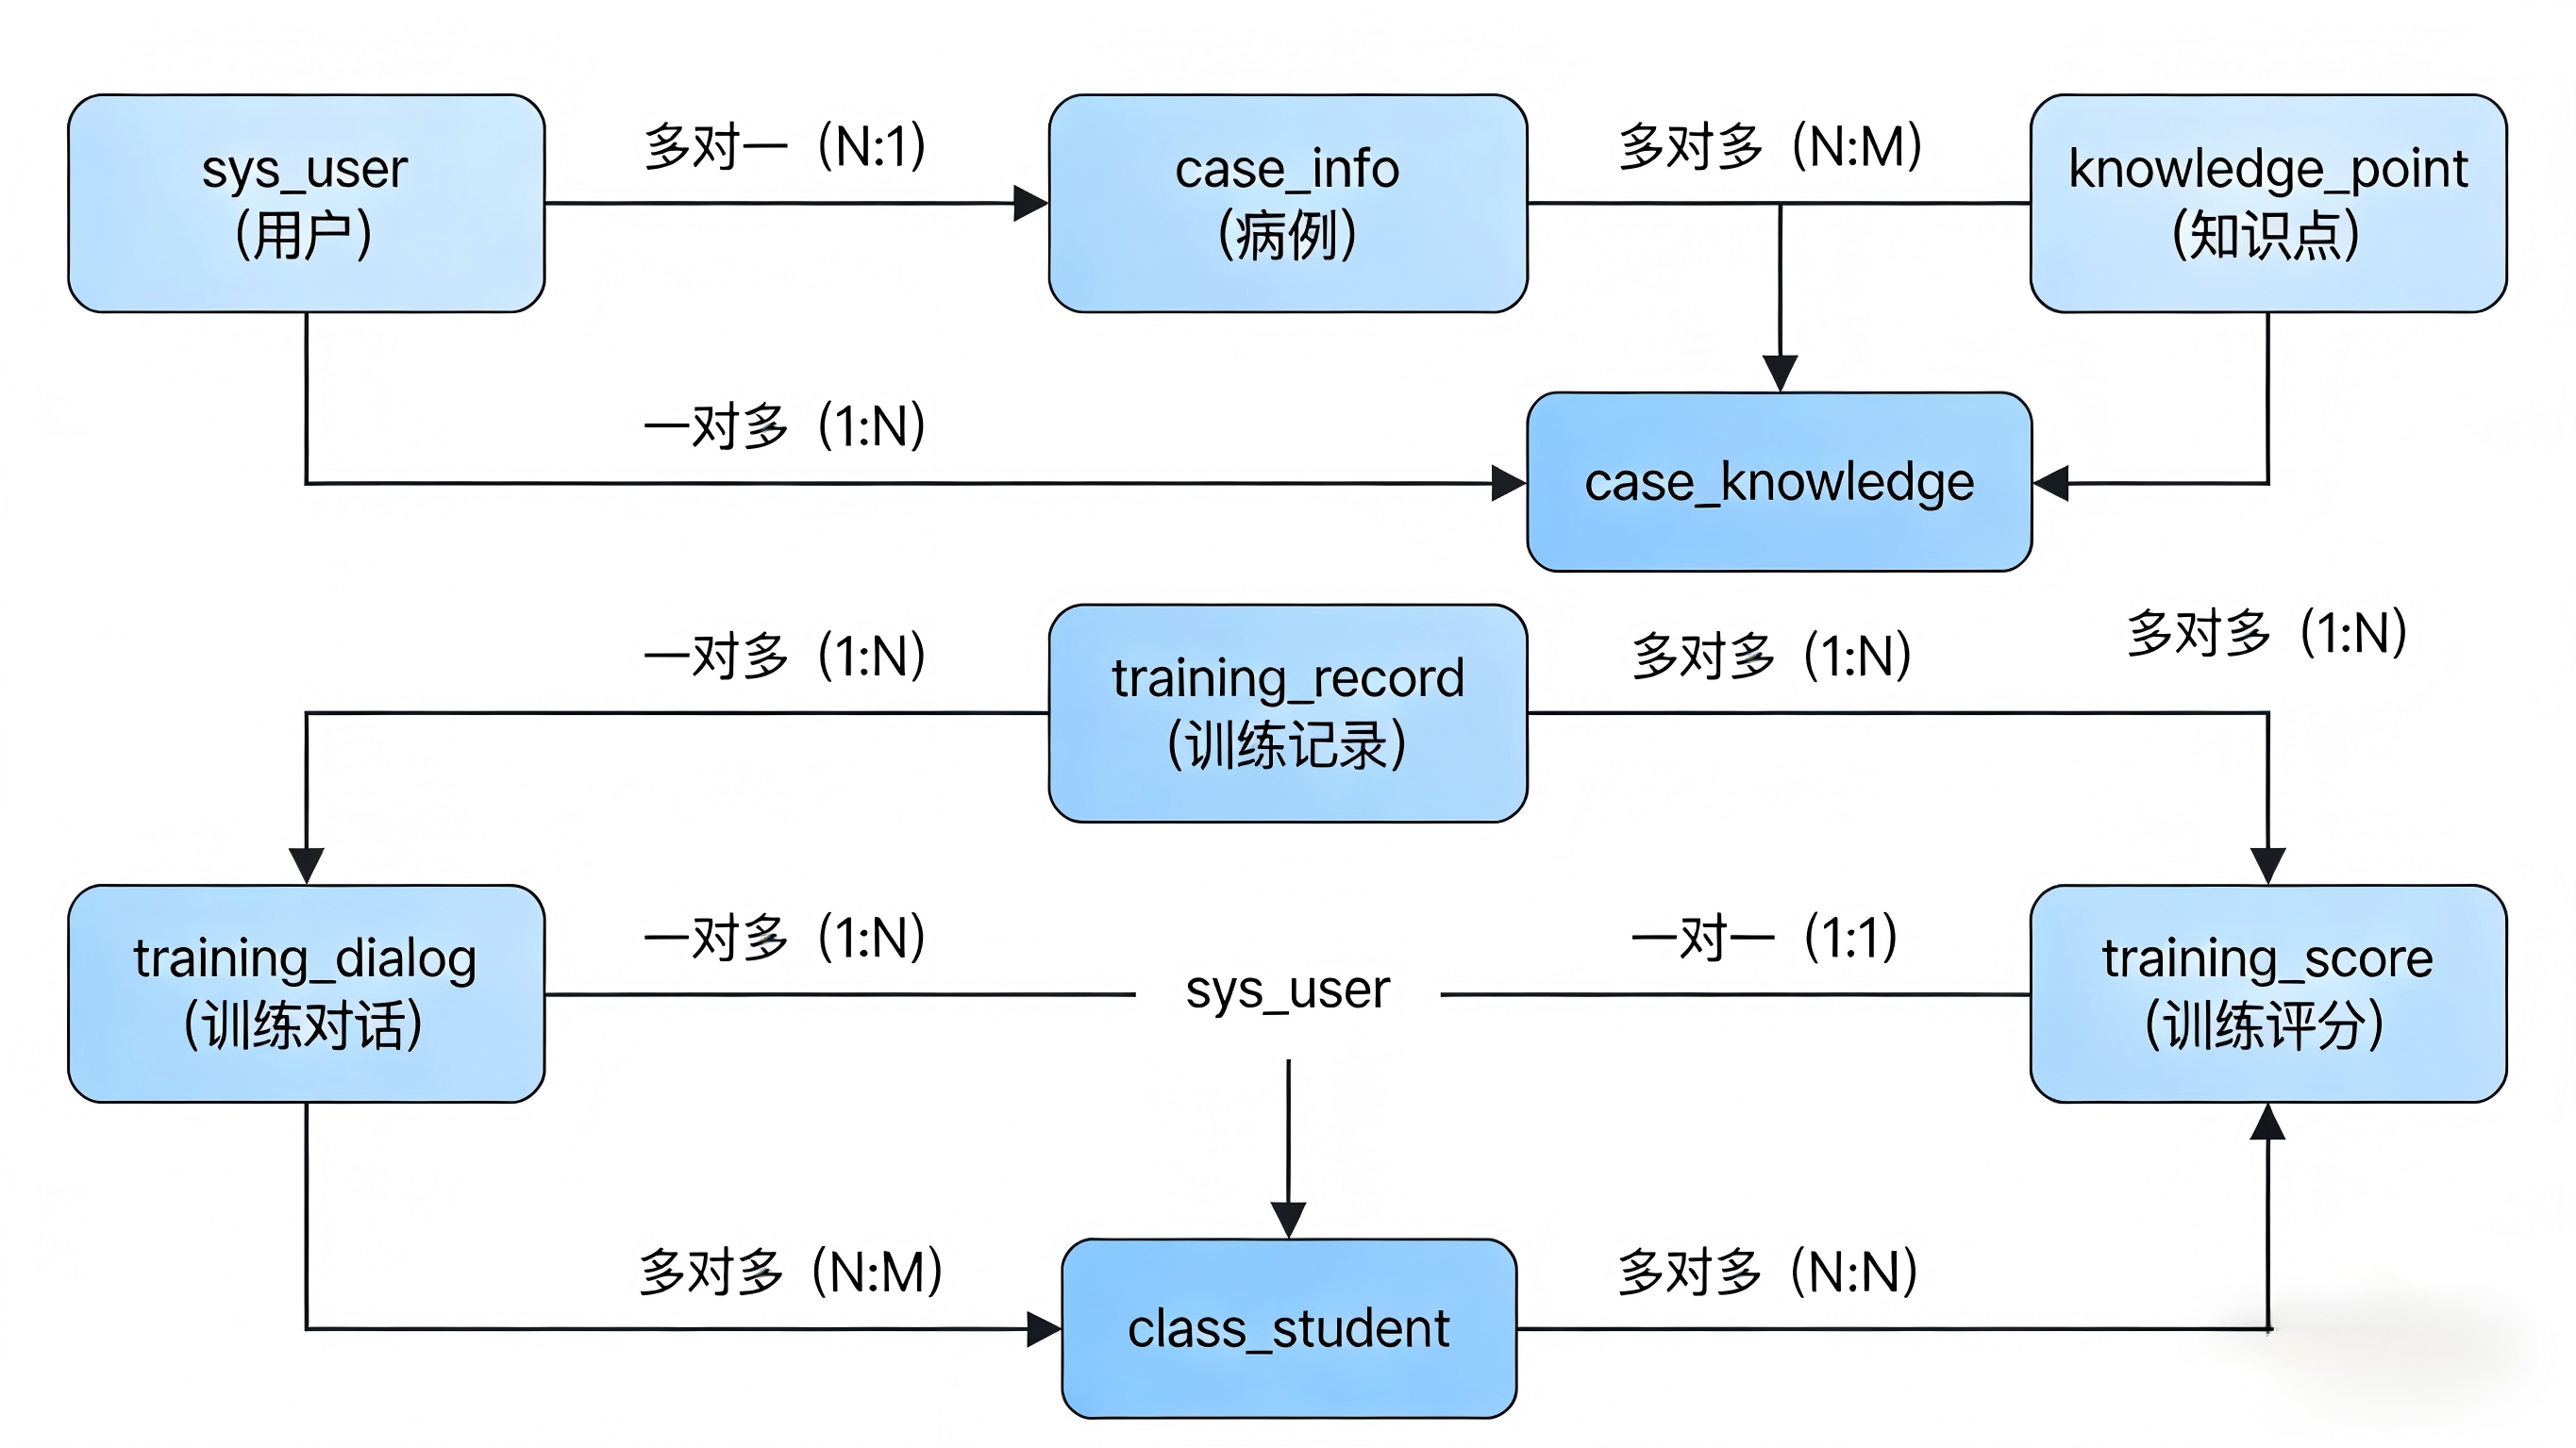
\includegraphics[width=0.9\textwidth]{figures/系统核心数据库ER图.png}
    \caption{系统核心数据库 ER 图}
    \label{fig:er_diagram}
\end{figure}

为直观展示上述实体在一次问诊训练中的运行时关系，图~\ref{fig:object_diagram} 给出了一个典型训练场景的 UML 对象图。

\begin{figure}[H]
    \centering
    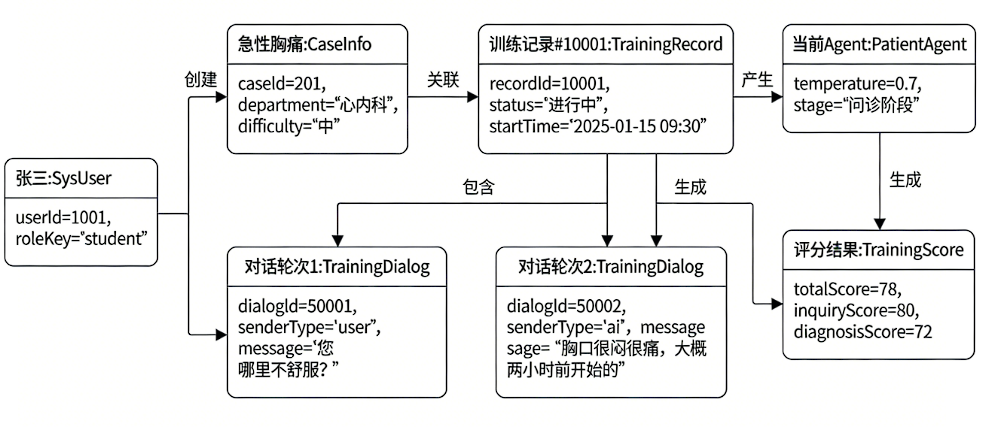
\includegraphics[width=0.85\textwidth]{figures/AI问诊训练运行时对象图.png}
    \caption{AI 问诊训练运行时对象图}
    \label{fig:object_diagram}
\end{figure}

\subsection{主要数据表设计}
系统采用 MySQL 8.0 作为核心业务数据库，字符集统一为 \texttt{utf8mb4}，以支持中文病例、医学术语与多语言文本。业务表普遍包含 \texttt{create\_time}、\texttt{update\_time}、\texttt{deleted} 等字段，便于审计和逻辑删除。考虑到本科毕业论文正文不宜堆叠过多字段明细，本节围绕系统主业务链路概括核心数据表的职责、关键字段和关系，如表~\ref{tab:core_tables} 所示。完整建表语句随项目源码资料提交。

\begin{table}[H]
    \centering
    \caption{核心业务数据表汇总}
    \label{tab:core_tables}
    \small
    \begin{tabularx}{\textwidth}{@{}p{2.7cm}p{2.8cm}X p{3.0cm}@{}}
        \toprule
        数据表 & 主要职责 & 关键字段 & 关联关系 \\
        \midrule
        用户表 & 用户身份与基础资料 & 登录名、密码哈希、角色、学号或工号、账号状态 & 多个用户对应一个角色 \\
        病例表 & 病例基础信息与 Agent 问诊依据 & 标题、科室、难度、主诉、参考诊断、参考治疗方案 & 教师创建病例，训练记录引用病例 \\
        训练记录表 & 一次问诊训练的主记录 & 学生、病例、训练状态、提交诊断、提交治疗方案 & 连接学生、病例、对话和评分 \\
        对话明细表 & 多轮问诊对话明细 & 训练记录、发送方、消息内容、消息类型、创建时间 & 一条训练记录对应多条对话 \\
        评分表 & AI 与教师评分结果 & 总分、问诊分、诊断分、治疗分、薄弱点、评分版本 & 一条训练记录对应一组评分 \\
        知识点表 & RAG 检索和学习分析知识库 & 标题、正文、分类、标签、错误次数 & 通过病例知识点关系与病例关联 \\
        班级相关表 & 班级管理与成绩统计范围 & 班级名称、专业、教师、学生、加入状态 & 教师按班级查看学生训练结果 \\
        \bottomrule
    \end{tabularx}
\end{table}

\subsection{Redis 数据结构}
Redis 在系统中承担临时状态、登录安全与 AI 对话上下文缓存的职责。与 MySQL 中的持久化训练记录不同，Redis 数据均设置 TTL 或可主动清理，避免对话中间态长期堆积。表~\ref{tab:redis_keys} 给出了系统中的主要 Redis Key 设计。

\begin{table}[H]
    \centering
    \caption{Redis 主要数据结构设计}
    \label{tab:redis_keys}
    \small
    \begin{tabularx}{\textwidth}{@{}p{3.7cm}p{1.9cm}p{1.9cm}X@{}}
        \toprule
        Key 模式 & 类型 & 过期策略 & 用途 \\
        \midrule
        \texttt{session:memory:}\newline\texttt{\{recordId\}} & String & 24 小时 & 保存某次训练最近若干轮对话上下文，供 Agent 拼接 Memory \\
        \texttt{captcha:\{sessionId\}} & String & 5 分钟 & 图形验证码校验，验证成功后立即删除 \\
        \texttt{login:attempt:}\newline\texttt{\{username\}} & String / Number & 30 分钟 & 登录失败次数统计，超过阈值后触发锁定 \\
        \texttt{login:lock:}\newline\texttt{\{username\}} & String & 30 分钟 & 账户临时锁定标记，用于防暴力破解 \\
        \texttt{email:code:\{email\}} & String & 短期 TTL & 邮件验证码，支撑注册和密码重置 \\
        \bottomrule
    \end{tabularx}
\end{table}

% ----------------------------------------------------------------------------
\section{接口设计}
后端接口统一以 \texttt{/api} 作为业务前缀，采用 JSON 作为主要数据交换格式。普通业务接口返回统一结构 \texttt{\{code, message, data\}}，其中 \texttt{code=200} 表示业务成功，认证失败返回 401，参数错误返回 400，系统异常返回 500。AI 流式对话接口因需要逐字输出，使用 \texttt{text/event-stream} 作为响应类型，前端通过 EventSource 或流式请求解析增量内容。

\begin{table}[H]
    \centering
    \caption{核心接口分组设计}
    \label{tab:api_groups}
    \begin{tabular}{l l p{7cm}}
        \toprule
        接口分组 & 代表路径 & 主要职责 \\
        \midrule
        认证接口 & \texttt{/api/auth/*} & 登录、注册、验证码、刷新令牌、退出、密码重置、用户信息维护 \\
        病例接口 & \texttt{/api/case/*} & 病例列表、病例详情、病例新增、编辑、删除、元数据和推荐病例 \\
        训练接口 & \texttt{/api/training/*} & 开始训练、结束训练、放弃训练、训练列表、训练详情、提交评估 \\
        对话接口 & \texttt{/api/chat/*} & 普通发送、SSE 流式对话、历史对话查询 \\
        AI 接口 & \texttt{/api/ai/*} & 通用 AI 对话、流式输出、训练评分评估 \\
        成绩接口 & \texttt{/api/grades/*} & 成绩列表、教师评价、批量评分、学生与班级统计、成绩导出 \\
        分析接口 & \texttt{/api/analysis/*} & 学生学习分析、教师教学分析、雷达图与趋势统计 \\
        管理接口 & \texttt{/api/admin/*} & 用户、角色、日志、监控、存储和通知管理 \\
        文件接口 & \texttt{/api/files/*} & 文件上传、对象预览、医学影像访问 \\
        \bottomrule
    \end{tabular}
\end{table}

以“发送一次 AI 问诊消息”为例，前端在已登录状态下调用 \texttt{POST /api/chat/send}，请求头携带 JWT，主体中包含训练记录编号、病例编号与用户消息。若调用 \texttt{POST /api/chat/stream/\{recordId\}}，后端会在校验训练归属后进入 Agent 编排流程，并通过 SSE 逐段返回 AI 回复。非流式接口的典型请求与响应结构如下：

\begin{lstlisting}[caption={AI 问诊消息接口请求与响应示例}, label={lst:chat_api}]
POST /api/chat/send
Authorization: Bearer <token>
Content-Type: application/json

{
  "recordId": 10001,
  "caseId": 1,
  "message": "请问您胸痛是从什么时候开始的？"
}

{
  "code": 200,
  "message": "操作成功",
  "data": {
    "recordId": 10001,
    "senderType": "ai",
    "message": "大概两个小时前开始的，突然胸口很闷、很痛。",
    "messageType": "text"
  }
}
\end{lstlisting}

% ----------------------------------------------------------------------------
\section{RBAC 权限模型设计}
权限模型采用经典 RBAC（Role-Based Access Control）思想，通过“用户—角色—权限”三层关系降低授权复杂度。当前数据库初始化脚本已经落地 \texttt{super\_admin}、\texttt{admin}、\texttt{teacher}、\texttt{student} 四类角色，其中超级管理员拥有全局权限，管理员负责用户、日志和系统资源管理，教师负责病例、班级、成绩与教学分析，学生负责病例训练与个人学习分析。任务书与需求分析中提到的 \texttt{teacher\_admin} 可作为后续扩展角色，用于跨班级、跨教师的教务管理场景。

权限粒度按菜单、按钮、接口三层设计。菜单权限决定前端路由是否可见，按钮权限控制页面内“新增、编辑、删除、导出、批量评分”等具体操作，接口权限由后端 Spring Security 与业务层二次校验共同完成。对于训练记录、班级成绩等存在数据归属关系的资源，系统还需在业务层根据 \texttt{user\_id}、\texttt{teacher\_id}、\texttt{class\_id} 进行数据范围限制，避免同级角色之间相互越权。

\begin{figure}[H]
    \centering
    \begin{tikzpicture}[
        every node/.style={font=\small},
        box/.style={draw, rounded corners=2pt, minimum width=2.5cm, minimum height=0.75cm, align=center},
        user/.style={box, fill=blue!8},
        role/.style={box, fill=green!10},
        perm/.style={box, fill=orange!12},
        arr/.style={-{Latex[length=2mm]}, thick}
    ]
        \node[user] (u) {用户\\sys\_user};
        \node[role, right=1.4cm of u] (r) {角色\\sys\_role};
        \node[perm, right=1.4cm of r] (p) {权限\\sys\_permission};
        \node[perm, above right=0.4cm and 1.0cm of p] (menu) {菜单权限};
        \node[perm, right=1.0cm of p] (button) {按钮权限};
        \node[perm, below right=0.4cm and 1.0cm of p] (api) {接口权限};

        \draw[arr] (u) -- node[above]{N:1} (r);
        \draw[arr] (r) -- node[above]{N:M} (p);
        \draw[arr] (p) -- (menu);
        \draw[arr] (p) -- (button);
        \draw[arr] (p) -- (api);
    \end{tikzpicture}
    \caption{RBAC 权限模型设计}
    \label{fig:rbac_model}
\end{figure}

% ----------------------------------------------------------------------------
\section{安全架构设计}
系统安全架构从身份认证、访问控制、数据保护、输入校验和审计追踪五个层面设计。身份认证层采用 JWT 令牌机制\cite{jones2015jwt}，后端通过 JWT 认证过滤器从请求头中解析令牌，校验通过后将用户信息写入 Spring Security 上下文。

登录入口叠加图形验证码与登录失败锁定机制。验证码存入 Redis，5 分钟后自动过期；同一用户名连续失败 5 次后写入锁定标记，锁定 30 分钟，以降低暴力破解风险。

访问控制层采用 Spring Security 的无状态会话策略，登录、注册、验证码、健康检查、文件预览等少数路径开放访问，其余接口默认要求认证。对于学生训练记录、教师班级成绩和管理员数据，系统在 Controller 之后的 Service 层继续校验资源归属，形成“认证 + 角色 + 数据范围”的组合防护。数据保护层对密码采用 BCrypt 单向哈希存储，对手机号、邮箱等敏感字段预留 \texttt{@Encrypted} 注解与 \texttt{AESUtil} 字段级加密能力；操作日志切面 \texttt{@OperationLog} 会对密码、token、验证码等敏感参数进行脱敏后写入 \texttt{operation\_log}。输入与接口层面，系统通过 DTO 校验、统一异常处理、MyBatis-Plus 参数化查询以及 Nginx 跨域策略降低 SQL 注入、越权调用与异常信息泄露风险。由于系统主要面向前后端分离的无状态 API，当前后端关闭 CSRF，并以 JWT、CORS 白名单和接口鉴权共同保障调用安全。

% ----------------------------------------------------------------------------
\section{本章小结}

本章在需求分析的基础上完成了系统总体设计，给出了分层架构、前后端分离方式、多 Agent 协同架构、功能模块划分、核心数据库模型、Redis 缓存结构、接口分组、RBAC 权限模型和安全架构。总体上，本系统并非简单地把大语言模型接入传统教学系统，而是在 Web 工程架构中单独抽象出 AI 服务层，使 Agent、RAG、Memory、工具调用和评分能力可以被训练、批改与学习分析复用。下一章将进一步展开 AI Agent 核心技术实现，说明系统如何将大语言模型改造为可控、可追踪、可评分的医学问诊训练引擎。
